% Created 2016-08-17 Wed 14:38
\documentclass[tikz]{standalone}

\usepackage[utf8]{inputenc}
\usepackage[T1]{fontenc}

\usepackage{circledsteps}

\RequirePackage{xcolor}

%% HPI color definitions according to the design manual
% These do not exactly match the RGB values used in the Powerpoint slide master due to unknown reasons
\definecolor{hpiyellow}{RGB}{246,168,0}
\definecolor{hpiorange}{RGB}{221,97,8}
\definecolor{hpired}{RGB}{177,6,58}
\definecolor{hpigray}{RGB}{90,96,101}
\definecolor{hpiblue}{RGB}{0,122,158}


\renewcommand{\sfdefault}{neosans}
% Different font weights for neosans
\newcommand{\textl}[1]{{\fontseries{l}\selectfont #1}} % light
\newcommand{\textm}[1]{{\fontseries{m}\selectfont #1}} % medium, same as default weight
\newcommand{\textsb}[1]{{\fontseries{sb}\selectfont #1}} % semibold
\newcommand{\textmb}[1]{{\fontseries{mb}\selectfont #1}} % bold, same as \textbf
\newcommand{\texteb}[1]{{\fontseries{eb}\selectfont #1}} % extra bold
\newcommand{\textub}[1]{{\fontseries{ub}\selectfont #1}} % ultra bold

\tikzset{every picture/.style={/utils/exec={\sffamily}}}
\tikzset{flipflop RSflanke/.style={
  flipflop,
  flipflop def={t1=S, t2=C, c2=1, t3=R, t6=Q, t4={\ctikztextnot{Q}}}
}}


\tikzset{
  mechanicalSwitch/.pic={
    \coordinate (-inUp) at (135:2); 
    \coordinate (-inDown) at (235:2);
    \coordinate (-out) at (2,0);
    \coordinate (-center) at (0,0);
    
    \draw (0,0) circle [radius = 2cm];
    \draw [fill=gray!20] (0,0) circle [radius = 0.2cm];

    \draw (0, 0) -- (2, 0);
    \draw (135:.8) -- (135:2); 
    \draw (225:.8) -- (225:2); 

    \draw [fill=gray!20] (2, 0) circle [radius=0.05cm]; 
    \draw [fill=gray!20] (135:2) circle [radius=0.05cm]; 
    \draw [fill=gray!20] (225:2) circle [radius=0.05cm]; 

    
    \draw [thick] (0,0) -- (175:1.5); 

    \draw [dashed, <->, domain=135:225] plot ({cos(\x)}, {sin(\x)}); 
  },
  mechanicalSwitchClosed/.pic={
    \coordinate (-inUp) at (135:2); 
    \coordinate (-inDown) at (255:2);
    \coordinate (-out) at (2,0);
    \coordinate (-center) at (0,0);
    \draw (0,0) circle [radius = 2cm];
    \draw [fill=gray!20] (0,0) circle [radius = 0.2cm];

    \draw (0, 0) -- (2, 0);
    \draw (135:.8) -- (135:2); 
    \draw (225:.8) -- (225:2); 

    \draw [fill=gray!20] (2, 0) circle [radius=0.05cm]; 
    \draw [fill=gray!20] (135:2) circle [radius=0.05cm]; 
    \draw [fill=gray!20] (225:2) circle [radius=0.05cm]; 

    
    \draw [thick] (0,0) -- (135:2); 

    \draw [dashed, <->, domain=135:225] plot ({cos(\x)}, {sin(\x)}); 
  }
}


\usetikzlibrary{calc}
\usetikzlibrary{positioning}


\usetikzlibrary{calc}

\usepackage{pgfplots}

\begin{document}

\pgfplotsset{every axis/.append style={
    font=\large,
    line width=1pt,
    tick style={line width=0.8pt}}}

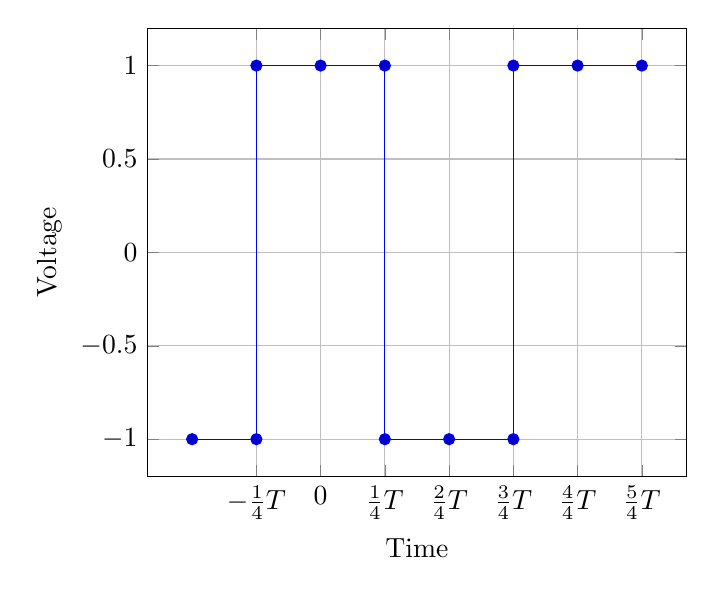
\begin{tikzpicture}
  \label{page:phy:simple_fourier}
  \begin{axis}
    [grid=major,
    xlabel=Time,
    ylabel=Voltage,
    xtick= {-1, 0, 1, 2, 3, 4,5},
    xticklabels={$-\frac{1}{4}T$,0,$\frac{1}{4}T$, $\frac{2}{4}T$, $\frac{3}{4}T$, $\frac{4}{4}T$, $\frac{5}{4}T$}]
    \addplot coordinates { (-2, -1) (-1,-1) (-1,1) (0,1) (1,1) (1, -1) (2,-1) (3, -1) (3,1) (4,1) (5, 1) };
  \end{axis}
\end{tikzpicture}


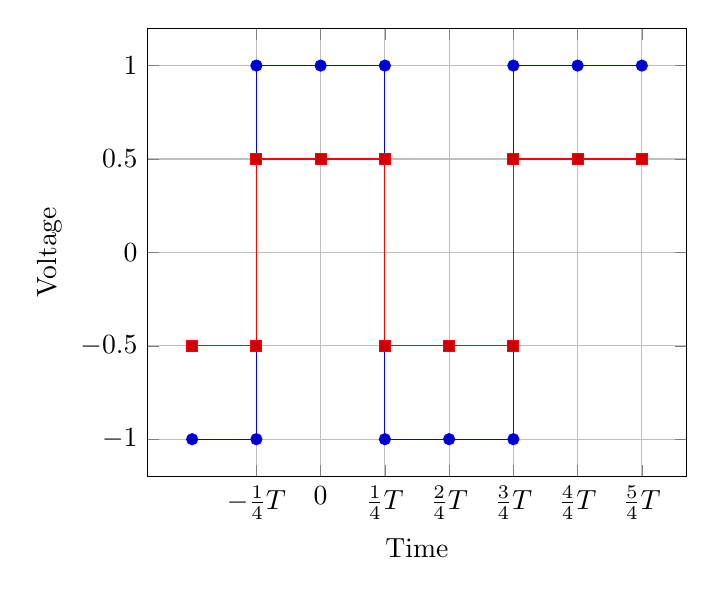
\begin{tikzpicture}
  \label{page:phy:attenuated_simple_fourier}
  \begin{axis}
    [grid=major,
    xlabel=Time,
    ylabel=Voltage,
    xtick= {-1, 0, 1, 2, 3, 4,5},
    xticklabels={$-\frac{1}{4}T$,0,$\frac{1}{4}T$, $\frac{2}{4}T$, $\frac{3}{4}T$, $\frac{4}{4}T$, $\frac{5}{4}T$}]
    \addplot  coordinates { (-2, -1) (-1,-1) (-1,1) (0,1) (1,1) (1, -1) (2,-1) (3, -1) (3,1) (4,1) (5, 1) };
    \addplot coordinates { (-2, -0.5) (-1,-0.5) (-1,0.5) (0,0.5) (1,0.5) (1, -0.5) (2,-0.5) (3, -0.5) (3,0.5) (4,0.5) (5, 0.5) };
  \end{axis}
\end{tikzpicture}


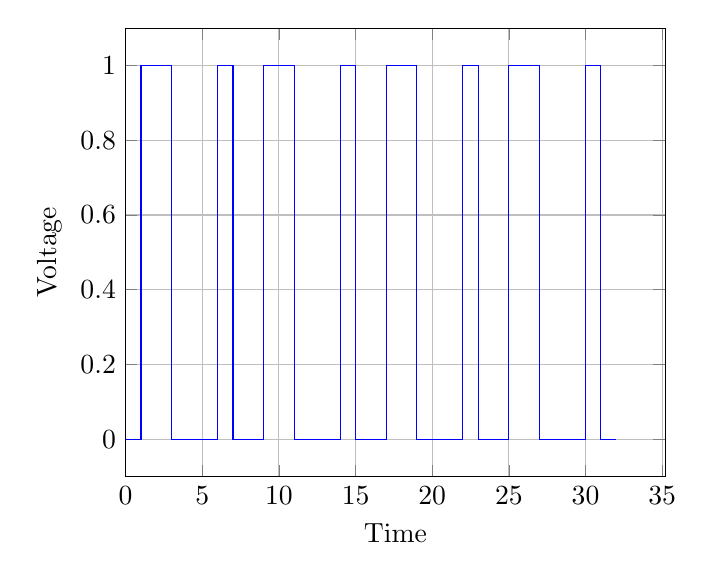
\begin{tikzpicture}
  \label{page:phy:repeated_fourier}
  \begin{axis}
    [grid=major,
    xlabel=Time,
    ylabel=Voltage,
    no markers,
    % xtick= {-1, 0, 1, 2, 3, 4,5},
    % xticklabels={$-\frac{1}{4}T$,0,$\frac{1}{4}T$, $\frac{2}{4}T$, $\frac{3}{4}T$, $\frac{4}{4}T$, $\frac{5}{4}T$}
    xmin=0
    ]
    \foreach \i in {0,1,2,3} {
      \addplot [blue] coordinates {
        (0+8*\i,0) (1+8*\i,0) (1+8*\i,1) (3+8*\i,1) (3+8*\i,0) (6+8*\i,0) (6+8*\i,1) (7+8*\i,1) (7+8*\i,0) (8+8*\i,0)
        % (0+8*\i,1) (1+8*\i,1) (1+8*\i, -1) (2+8*\i,-1) (3+8*\i, -1) (3+8*\i,1) (4+8*\i,1)
      };
      }
  \end{axis}
\end{tikzpicture}






\end{document}